\documentclass[b5paper]{standalone}
\usepackage{fontspec}
\usepackage{polyglossia}
\usepackage{tikz}
\usepackage{ifthen}   
\usepackage{amsmath}
\usepackage{graphics}
\usepackage{siunitx}
\usetikzlibrary{calc}
%
\setmainlanguage{english}
\setotherlanguages{arabic}
\newfontfamily\arabicfont[Scale=1.0,Script=Arabic]{Scheherazade}
\newfontfamily\urdufont[Scale=1.0,Script=Arabic]{XB Tabriz}

\begin{document}
\begin{urdufont}
\begin{tikzpicture}
    \node[anchor=south west,inner sep=0] (image) at (0,0) {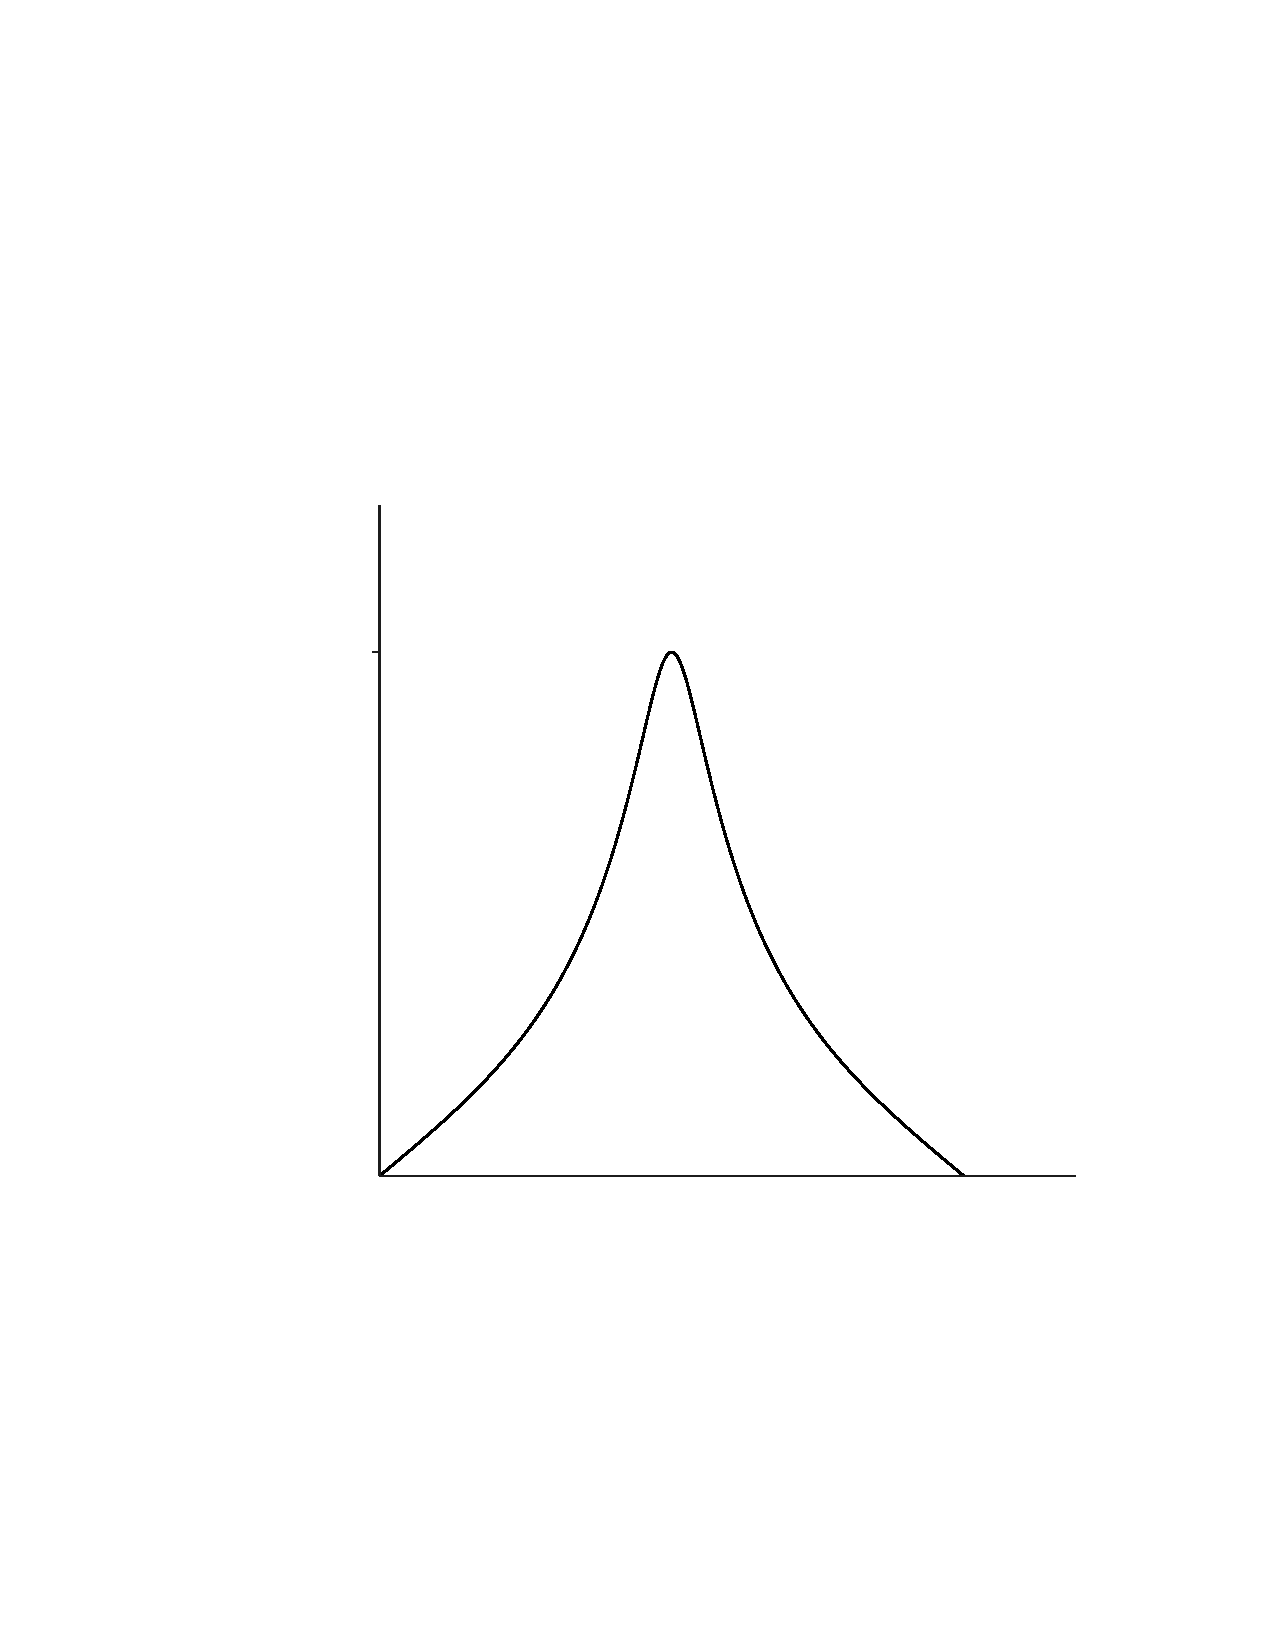
\includegraphics[height=2.5cm,trim={1cm 7cm 0cm 8cm},clip]{figExcitationCurrentFromBHbrillouinCurveNeglectingHysterisis}};
    \begin{scope}[x={(image.south east)},y={(image.north west)}]
%grid
%\draw [gray, thick,xstep=0.1,ystep=0.1] (0,0) grid (1,1);
%\draw [gray, thin,xstep=0.01,ystep=0.01] (0,0) grid (1,1);

\node at (0.07,0.75){\SI{0.667}{\ampere}};
\node at (0.2,0.97){$i_\varphi$};
\node at (0.95,0.05){$t$};
\node at (0.74,-0.08){$\frac{\pi}{\omega}$};
    \end{scope}
\end{tikzpicture}
\end{urdufont}
\end{document}

